\documentclass[12pt]{article}
\usepackage{latexsym,amssymb,amsmath} % for \Box, \mathbb, split, etc.
% \usepackage[]{showkeys} % shows label names
\usepackage{cite} % sorts citation numbers appropriately
\usepackage{path}
\usepackage{url}
\usepackage{verbatim}
\usepackage[pdftex]{graphicx}
\usepackage{color}

\usepackage{multicol}
\usepackage{fullpage}

% horizontal margins: 1.0 + 6.5 + 1.0 = 8.5
\setlength{\oddsidemargin}{0.0in}
\setlength{\textwidth}{6.5in}
% vertical margins: 1.0 + 9.0 + 1.0 = 11.0
\setlength{\topmargin}{0.0in}
\setlength{\headheight}{12pt}
\setlength{\headsep}{13pt}
\setlength{\textheight}{625pt}
\setlength{\footskip}{24pt}

\renewcommand{\textfraction}{0.10}
\renewcommand{\topfraction}{0.85}
\renewcommand{\bottomfraction}{0.85}
\renewcommand{\floatpagefraction}{0.90}

\makeatletter
\setlength{\arraycolsep}{2\p@} % make spaces around "=" in eqnarray smaller
\makeatother

% change equation, table, figure numbers to be counted inside a section:
\numberwithin{equation}{section}
\numberwithin{table}{section}
\numberwithin{figure}{section}

% begin of personal macros
\newcommand{\half}{{\textstyle \frac{1}{2}}}
\newcommand{\eps}{\varepsilon}
\newcommand{\myth}{\vartheta}
\newcommand{\myphi}{\varphi}

\newcommand{\IN}{\mathbb{N}}
\newcommand{\IZ}{\mathbb{Z}}
\newcommand{\IQ}{\mathbb{Q}}
\newcommand{\IR}{\mathbb{R}}
\newcommand{\IC}{\mathbb{C}}
\newcommand{\Real}[1]{\mathrm{Re}\left({#1}\right)}
\newcommand{\Imag}[1]{\mathrm{Im}\left({#1}\right)}

\newcommand{\norm}[2]{\|{#1}\|_{{}_{#2}}}
\newcommand{\abs}[1]{\left|{#1}\right|}
\newcommand{\ip}[2]{\left\langle {#1}, {#2} \right\rangle}
\newcommand{\der}[2]{\frac{\partial {#1}}{\partial {#2}}}
\newcommand{\dder}[2]{\frac{\partial^2 {#1}}{\partial {#2}^2}}

\newcommand{\nn}{\mathbf{n}}
\newcommand{\xx}{\mathbf{x}}
\newcommand{\uu}{\mathbf{u}}

\newcommand{\junk}[1]{{}}

% set two lengths for the includegraphics commands used to import the plots:
\newlength{\fwtwo} \setlength{\fwtwo}{0.45\textwidth}


\renewcommand{\labelitemi}{}
\renewcommand{\labelitemii}{}
\renewcommand{\labelitemiii}{}


% end of personal macros
% \input{inputFile.tex}


\begin{document}
\DeclareGraphicsExtensions{.jpg}



\begin{center}
\textbf{\Large AAAI Fellowship Application}\\[12pt] 
%\textbf{\Large } \\[6pt]
%\textbf{\Large } \\[6pt]
John Oberlin\\
Brown University, 2014\\
\end{center}

\section{Dissertation Abstract}
Imagine handing ten everyday objects to your robot assistant, who then proceeds to
scan them and put them where they belong. Now think of a situation where a capable
robot might improve someone's life by helping a disabled person prepare a meal,
fetching a purse or storing a book for a bedridden patient, or handing ointment
to a busy parent whose hands are full taking care of their child.

State of the art techniques in object detection and pose estimation
are powerful and general but usually run at a rate much less than 1 Hz and require
time and expertise to build, maintain, and operate. The high demands of modern systems
can make it difficult to employ such techniques in real-time human-robot interaction.
Although effective solutions exist for category recognition, there is no off-the-shelf
framework for object detection, segmentation and pose estimation that allows new objects
to be quickly and easily added by non-experts.

The aim of my dissertation at Brown is to enable a robot
to autonomously scan 10 novel objects in order to construct robust models for detection,
pose estimation, grasping, and manipulation of those objects during collaborations with
a human operator. We propose the following workflow for this task: 1.) A human operator provides
the robot with a box of objects. 2.) The robot picks up each object and scans it from many different
perspectives to collect appearance data. 3.) The robot trains classifiers to recognize each object. 
4.) The robot collects labels and metadata for the objects from Amazon Mechanical Turk. 5.) The
robot can detect the objects in the environment and accurately respond to an operator's request
to fetch an object or put it away.

Popular techniques for real time detection use modified deformable part models (DPMs) \cite{kostas1} \cite{forsyth1},
and sometimes exploit different channels of data \cite{dietr1} \cite{sliding1}.  
These approaches have seen success in their target domains, but are too technical for general
application and need to be integrated with interactive systems. A computer 
vision system that is simple, reliable, and easy to use with ROS (Robot Operating System)
would benefit many researchers.

Our prototype system detects and estimates poses of objects in RGB-D video taken with a Kinect and
runs at a frequency of 2 Hz. Our detection framework
% uses a box metaphor to talk about space in a way that is amenable to 
calculates three quantities for each frame $f$ which facilitate
planning and reasoning. 

The first quantity is a subset $\mathcal{G}_f$ of pixel locations, which induces a grid graph whose nodes
correspond to locations spaced 5 pixels apart in the input image $f$ and whose edges connect each pixel to its
four cardinal neighbors in the grid. A pixel $g$ is included in $\mathcal{G}_f$ if the local average Objectness (see below)
exceeds a threshold. We manually tune the threshold at the moment, but it would be natural to use a
max-entropy approach such as herding \cite{herding} to adaptively control it.
The second quantity is $\mathcal{B}_f$, a list of the connected components of the graph induced by $\mathcal{G}_f$.
The third quantity is $\mathcal{R}_f$, a labeling which associates with each point $g \in \mathcal{G}_f$ a token
corresponding to the object instance depicted at that pixel location.

In other words, $\mathcal{G}_f$ denotes areas in the image that probably belong to an object, 
$\mathcal{B}_f$ describes clusters of pixels which likely correspond to individual objects, and $\mathcal{R}_f$
segments $\mathcal{G}_f$ into object instances, which may involve breaking apart the clusters in $\mathcal{B}_f$.

We determine $\mathcal{G}_f$ using an Objectness measure \cite{bing}, extract features with SIFT \cite{sift} 
and k-means, and perform k-nearest neighbors classification on crops $C_B$ and $C_R$ induced by 
$\mathcal{B}_f$ and $\mathcal{R}_f$. 
We currently optimize the objective function for $\mathcal{R}_f$ using a variant of the wide-scale random noise algorithm \cite{wsrn}.
We publish detections and pose estimates in ROS for the crops $C_B$ and $C_R$. 

To provide accurate help
to a human partner, the robot needs to know how to manipulate objects and understand their typical uses.
Our system will address this issue by inferring object affordances and inducing an OO-MDP \cite{OOMDP} that the robot
can use for robust planning and object manipulation.

We might achieve better performance when determining $\mathcal{R}_f$
by using more sophisticated techniques that incorporate feedback with the robot's OO-MDP planner in 
order to collect additional, specific data as it is needed.  
Employing a POMDP \cite{POMDP} to explore the space of bounding boxes is a natural approach to investigate.

\begin{figure}
  \begin{center}
    \begin{tabular}{l c}
      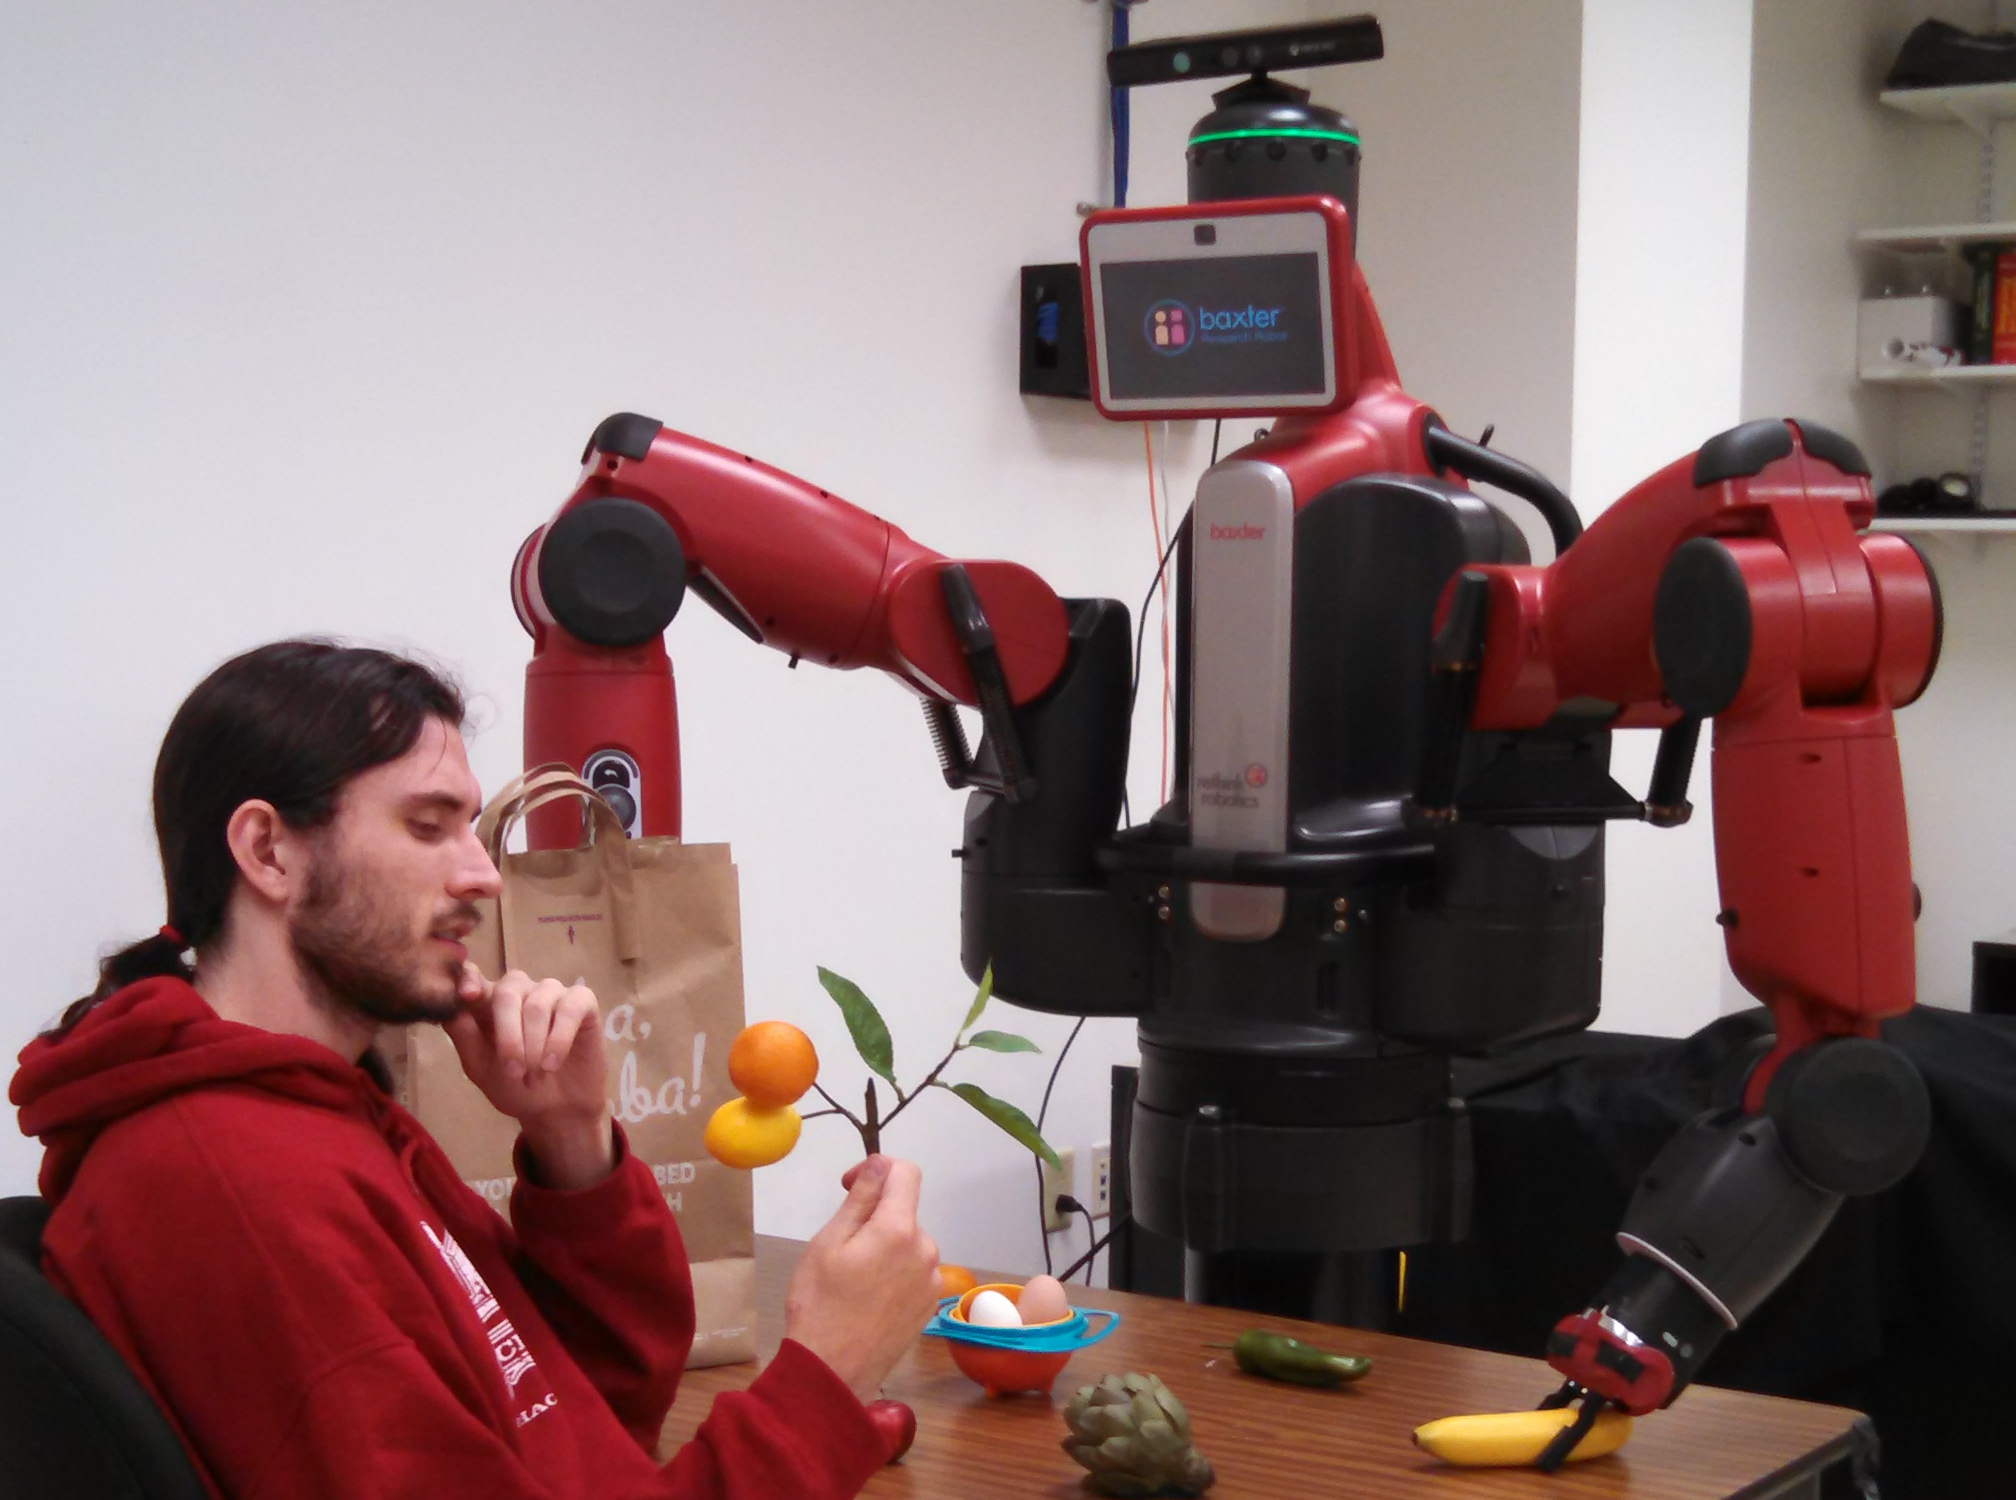
\includegraphics[width=200px, height=150px]{robo2.png} &
      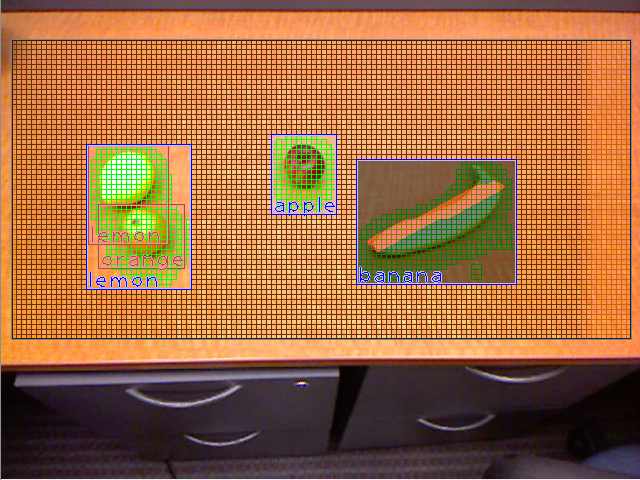
\includegraphics[width=200px, height=150px]{screen2.png} \\
    \end{tabular}
  \end{center}
  \caption{Teaching a robot to identify and manipulate objects can be as easy as bringing home
	    a bag of groceries.}
\end{figure}

%\paragraph{Semi-Automatic Training}
%\begin{enumerate}
  %\item A human operator places the object in a robot's manipulator.
  %\item The operator provides a base pose for the given grasp.
  %\item The robot collects views of many different precisely known poses, together with models for self and background filtering.
%\end{enumerate}

With our prototype system, a computer vision researcher can train accurate models for 5
objects in 15 minutes. Our aim is to integrate a robot into the workflow so that a novice
user can train 10 objects with 5 minutes of human input.

The system we have outlined abstracts the detector from the classifier, taking the notion of Objectness and
extending it. As more sophisticated computer vision algorithms become tractable in real time or new data becomes
available, they might be smoothly incorporated into the system even as it is running. 
Automatic model validation can ensure that a new model outperforms the current model before the system switches 
it out with no interruption of service. This technology will enable robots to help people by robustly sensing and
manipulating the objects that people value most.

\newpage

\bibliographystyle{siam}
\bibliography{proposal}

\newpage

\section{Attendance Statement}
   Work in computer vision has largely centered around specific problems concerning
single images. This focus has resulted in significant progress on such tasks, but the challenges of 
engineering real time systems has so far prevented all but a handful of methods from spreading 
to other communities. At one time it was said that AI was ``vision hard" and that solving vision would
effectively solve AI. While that belief sweeps a bit under the rug, it is certainly true
that in the past computer vision has been a strong bottleneck in the development of AI and 
robotics. 

There are now many techniques in computer vision which are suited
to fast and effective partial solutions of problems such as object detection
but have been ignored in favor of much slower but slightly more effective state of the art
approaches.  Such techniques may be combined with the information available from
extra sensors and the ability of real time systems to capture additional images of the same scene
to form full solutions to multiple related problems (such as detection, segmentation, and pose estimation). 

Recent advances in object detection on large data sets suggest that we are ready
to move beyond attacking vision in an isolated setting and begin integrating it in a
larger framework for planning in an interactive environment. 
 
I recently joined a robotics lab, so despite my strong training in computer vision,
there are still a few gaps in my background that I would like to fill.
By attending AAAI I will be able to better provide computer vision capabilities in a
way that is compatible with AI formalisms, researchers, and systems.

\newpage

\section{Curriculum Vitae}
\textbf{\emph{Education}}\\
 \\
BS in Math, Florida State University, 2003-2006 \\
MA in Math, UC Berkeley, 2006-2008 \\
PhD program in Computer Science at U Chicago, 2010-2011 \\
PhD program in Computer Science at Brown University, 2011-Present \\
 \\ 
\textbf{\emph{Employment}}\\
\\
Developer Support Engineer, Havok, 2008-2009 \\
 \\
\textbf{\emph{Conference Papers}}\\
 \\
S. Naderi Parizi, J. Oberlin, P. Felzenszwalb.\\
\emph{Reconfigurable Models for Scene Recognition.}\\
IEEE Conference on Computer Vision and Pattern Recognition (CVPR), 2012\\
 \\
P. Felzenszwalb, J. Oberlin.  \\
\emph{Multiscale Fields of Patterns.}\\
To Appear, 2014 \\
 \\
\textbf{\emph{Conferences Attended}}\\
 \\
CVPR 2011\\
CVPR 2012 \\
 \\
\textbf{\emph{Teaching Experience}}\\
 \\
Being a TA in the UCB Math Deparment can be close to a full time teaching position, including
quiz design, office hours, and grading in addition to the intense recitation sections (which more closely resembled lectures). \\
\\
Calculus 1 TA\\
UC Berkeley, 2006-2007\\
Two sections in the Fall, three sections in the Spring, 30 students in each section, each section met with me
two or three times a week for a total of about three hours a week.\\
 \\
Linear Algebra and ODE TA\\
UC Berkeley, 2007-2008\\
Same configuration as calculus.\\
 \\
Algorithms Grad TA\\
Brown University, 2012-Present\\
\\
I am currently the Grad TA for the Algorithms class at Brown for the fourth semester. During this time the class has been
between 45 and 100 students each iteration.  I have been responsible for administering oral exams, holding office hours,
lots of grading (most of our problems are proof based), and managing a group of at least 6 Undergraduate TA's each semester.\\
 \\
\textbf{\emph{Departmental Service}}\\
 \\
Graduate Student Orientation Leader\\
Brown CS Department, Fall 2012\\
 \\
Computer Vision Reading Group Coordinator\\
Brown CS Department, 2012\\
 \\
Department Tea Organizer\\
Brown CS Department, 2012-Present\\
 \\
\textbf{\emph{Misc Research}}\\
 \\
Master's Thesis in Mathematics\\
UC Berkeley, Written 2006-2008\\
 \\
Research Experience for Undergraduates in Mathematics\\
Oregon State University, Summer 2005\\
 \\
Undergraduate Research Program in Physics\\
Florida State University, Summer 2004\\
 \\
Research Assistant in Molecular Biology\\
Florida State University, Summer 2003\\
 \\
\textbf{\emph{Hobbies}}\\
 \\
Gardening\\
Ballroom Dance\\
Martial Arts\\
Blacksmithing\\
3D Printing\\
 \\

\end{document}

